%\documentclass[14pt]{article}
%\usepackage[margin=0.5in]{geometry}

\documentclass[a4paper,twoside,11pt]{article}
\usepackage[margin=3cm]{geometry}

\usepackage{lingmacros}
\usepackage{tree-dvips}
\usepackage{url}

\usepackage{pgfplotstable}
\usepackage{pgfplots}
\pgfplotsset{compat = 1.3}
\usepackage{subfig}

\usepackage{amssymb}
\setcounter{tocdepth}{3}
\usepackage{graphicx}

\usepackage{times}
\usepackage{graphicx}
\usepackage{latexsym}
\usepackage{algorithm}
\usepackage{float}
\usepackage[noend]{algpseudocode}
\usepackage{amssymb}
\usepackage{amsmath,amsthm} 
\usepackage{amsfonts}
%%%%%%%\usepackage{mathtools}
\usepackage{verbatim} 
\usepackage{longtable}
\usepackage{graphicx}
\usepackage{booktabs}
\usepackage{epstopdf}
\usepackage{longtable}
\usepackage{pgfpages}
\usepackage{multirow}
\usepackage{varwidth}
\usepackage{tabularx} % for aligning & numbering equations on the same line
\usepackage{enumitem}
\usepackage{pifont}
\usepackage{textcomp} % for ~

\usepackage{amsthm,amssymb,amsmath}
\usepackage{helvet,times,courier}
\usepackage{listings}
\usepackage[pdfborder={0 0 0},pagebackref=true]{hyperref}
\usepackage{fancyvrb}
\usepackage{fancyhdr}

\definecolor{pdBlue}{HTML}{748AAF}
\definecolor{pdGrey}{HTML}{898488} 
\definecolor{pdOrange}{HTML}{FF9934} 
\definecolor{pdDarkOrange}{HTML}{E14900}
\definecolor{pdDarkRed}{HTML}{230100}
\colorlet{InitMarkColour}{black!50!green}
\colorlet{TermMarkColour}{red}

\definecolor{plotRed}{HTML}{D25964}
\definecolor{plotBlue}{HTML}{3F6CAF}

\colorlet{darkGreen}{black!70!green}
\colorlet{darkRed}{black!50!red}
\colorlet{darkBlue}{black!50!blue}

\newcommand{\code}[1]{\color{purple!90!black}\texttt{#1}\color{black}}
\newcommand{\inputcmd}[1]{\color{darkGreen}\texttt{\textbf{#1}}\color{black}}
\newcommand{\cmdout}[1]{\color{darkBlue}\texttt{#1}\color{black}}
\newcommand{\logcode}[1]{\textsf{#1}}

\newcommand{\trail}{\textsf{\small TRAIL}}
\newcommand{\trailrun}{\texttt{\small trailrun}}
\newcommand{\trailhome}{\texttt{\$TRAIL\_HOME}}
\newcommand{\clingo}{\textsf{\small Clingo}}
\newcommand{\lomrf}{\textsf{\small LoMRF}}
\newcommand{\learnrev}{\textsf{\small LearnRevise}}
\newcommand{\xhail}{\textsf{\small XHAIL}}
\newcommand{\iled}{\textsf{\small ILED}}
\newcommand{\oled}{\textsf{\small OLED}}
\newcommand{\woled}{\textsf{\small WOLED}}

\theoremstyle{definition}
\newtheorem{texample}{Example}[section]
\newtheorem{tremark}{Remark}[section]

\newenvironment{remark}{\begin{tremark}}{\hfill$\blacksquare$\end{tremark}}
\newenvironment{example}{\begin{texample}}{\hfill$\blacksquare$\end{texample}}

%\title{Temporal Relational Theory Learning: \\ The \textsf{TRAIL} \ System Manual}
%\date{}
%\author{Nikos Katzouris \\ Institute of Informatics \& Telecommunications,\\Natinal Center for Scientific Research ``Demokritos''\\
%\url{nkatz@iit.demokritos.gr}}

\newcommand{\HRule}[1]{\rule{\linewidth}{#1}} 	% Horizontal rule

\makeatletter							% Title
\def\printtitle{%						
	{\centering \@title\par}}
\makeatother									

\makeatletter							% Author
\def\printauthor{%					
	{\centering \large \@author}}				
\makeatother							

% --------------------------------------------------------------------
% Metadata (Change this)
% --------------------------------------------------------------------
\title{	%\normalsize \textsc{Title page subtitle} 	% Subtitle
	%\\[2.0cm]								% 2cm spacing
	\HRule{0.5pt} \\
	[0.5cm]						% Upper rule
	\LARGE \textbf{Temporal Relational Theory Learning:\\ 
		The \textsf{TRAIL} System Manual}	\\
	[0.5cm]
	%\large Version 1.0 \\
	\large \url{https://github.com/nkatzz/ORL} \\
	\HRule{0.5pt} \\ [0.5cm]		% Lower rule + 0.5cm spacing
	\normalsize \today			% Todays date
}

\author{
	\Large Nikos Katzouris,\\	
	\normalsize
	Institute of Informatics \& Telecommunications,\\	
	National Center for Scientific Research ``Demokritos''\\
	\texttt{nkatz@iit.demokritos.gr} \\
}



\begin{document}	
%\pagestyle{plain}
%\maketitle

\thispagestyle{empty}		% Remove page numbering on this page

\printtitle					% Print the title data as defined above
%\vfill
\vspace*{3cm}
\printauthor				% Print the author data as defined above
%\newpage

\newpage
\pagestyle{plain} % fancy
\tableofcontents
\listoffigures
\newpage
\section{Introduction}
\label{sec:intro}

This document is intended to be used as a manual for \trail, a software package that provides a common interface to a number of \& algorithms for Temporal Relational Theory Learning. These algorithms are designed for learning logical theories from data of temporal nature, based on techniques from the fields of Inductive Logic Programming (ILP) \cite{de2008logical} \& Statistical Relational Learning (SRL) \cite{raedt2016statistical}. The learnt models may be used for reasoning with time \& events, in applications such as Complex Event Recognition (CER) \cite{cugola2012processing}. 

CER systems detect occurrences of \emph{complex events} in streaming input, defined as spatio-temporal combinations of \emph{simple events} (e.g. sensor data), using a set of complex event patterns. Since such patterns are not always known beforehand, while existing ones may frequently need to be updated to reflect change in the incoming data characteristics, machine learning algorithms for discovering such patterns from data are highly useful. Several challenges are involved in this type of learning. Scalability is a major requirement, since data collected in applications of temporal nature usually come in large volumes, or even in open-ended data streams. Also, such algorithms should be resilient to noise \& uncertainty, which are ubiquitous in temporal data sources \cite{DBLP:journals/corr/AlevizosSAP17}, while taking into account commonsense phenomena \cite{mueller2014commonsense}, which often characterize dynamic application domains. Finally, Valuable existing expert knowledge about the domain may greatly facilitate learning \& reasoning for CER if taken into account. This calls for expressive, yet highly efficient from an operational perspective, event pattern specification languages that allow to easily encode domain principles into usable background knowledge for learning \& reasoning. 

The learning algorithms contained in \trail \ attempt to address some of these challenges. Following work in logic-based approaches to CER \cite{artikis2012logic,artikis2015event}, which use first-order logic as a unifying representation language for events, complex event patterns and background knowledge, \trail \ is also based on logic. This allows for direct connections to machine learning techniques from the fields of ILP and SRL. A lot of work behind most of the learning algorithms in \trail \ has been devoted to scalability, with a focus on theory revision techniques, incremental \& online learning.\\

\noindent The following algorithms are implemented in \trail:

\begin{itemize}
	\item \learnrev, which is based on ideas from non-monotonic ILP and incorporates machinery from the \xhail \ \cite{ray2009nonmonotonic} algorithm, in addition to theory revision techniques. \learnrev \ operates in a ``one-shot'' mode, generalizing from a (typically small) excerpt of data, representative of some application domain. \learnrev \ is able to either learn a theory from scratch or revise an existing one.
	
	\item \iled, originally introduced in \cite{katzouris2015incremental}, an algorithm that lifts the non-monotonic learning \& theory revision techniques on which \learnrev \ relies to an incremental learning setting, in order to foster scalability. \iled \ learns incrementally, by iteratively processing small data ``snapshots'' (each such snapshot may be e.g. a small data chunk that \learnrev \ uses for one-shot learning). The \iled \ algorithm introduced in \cite{katzouris2015incremental} was designed for learning sound hypotheses (i.e. theories that correctly account for the entirety of the training data). It is thus not capable to deal with noise, which often makes it less useful in real-life applications. In contrast, although closely related to the original \iled \ algorithm, the  \iled \ version  included in \trail \ abandons the requirement for soundness and instead attempts to learn a theory that minimizes the training error, using theory revision techniques and an iterative hill-climbing search in the space of theories. 
	\item \oled, an algorithm introduced in \cite{DBLP:journals/tplp/KatzourisAP16}, which learns logical theories in an online fashion, i.e. in a single-pass over a training set. 
	
	\item \woled, an algorithm introduced in \cite{kr2020}, which learns learns rules' structure \& weights in an online fashion. \woled \ is also capable of probabilistic inference with the weighted rules.     
\end{itemize} 

\noindent \trail \ is based on Answer Set Programming (ASP) \cite{lifschitz2019answer} and all learning algorithms contained in this software package rely on the \clingo\footnote{\url{https://potassco.org/clingo/}} \ \cite{gebser2015potassco} answer set solver. 

This document contains some material on Inductive Logic Programming, Statistical Relational Learning and Answer Set Programming, but it is by no means an adequate introduction to any of these fields. The interested reader should refer to (e.g.) the books on these topics mentioned above (\cite{de2008logical,raedt2016statistical,lifschitz2019answer}), or to some other of the numerous resources that are available. The research papers mentioned earlier (and in what follows in this document) may also be helpful. More resources on CER may be found at the website of NCSR's Complex Event Recognition group\footnote{\url{http://cer.iit.demokritos.gr/}}. \textbf{All examples used throughout this document may be downloaded from...}  

The rest of the document is structured as follows: In Section...

\section{Installation}
\label{sec:install}
In order to build \trail \ from source you need to have a JDK installed (e.g. OpenJDK, or OracleJDK), version 8 or higher. You will also need SBT, the Scala Build Tool\footnote{\url{https://www.scala-sbt.org/}} (version 1.3.9 has been used with the code). \trail \ relies on the \clingo \ ASP solver\footnote{\url{https://potassco.org/clingo/}}. At the time of writing the latest \clingo \ release is v5.4.0. \trail \ won't work with \clingo \ version prior to v5.x.x. Due to the fact that \clingo's API is also used in \trail, Python 2.7 is also required to use the software.  

\subsection{Building \trail \ from Source}

The source code comes with an installation script, which takes care of several dependencies that are necessary for \clingo \ v5.4.0, as well as \clingo \ itself. The script also installs \lomrf\footnote{\url{https://github.com/anskarl/LoMRF}}, a library for Markov Logic Networks, which is used by some algorithms in \trail, mostly in order to compare Markov Logic-based to ASP-based tools for statistical relational learning. Using the script is the easiest way to install \trail. It has been tested on Ubuntu 18.04, but it should work on other Linux distributions that use apt for package management. If you encounter problems running the script it is recommended that you first try to install \clingo \ manually, by building it from source. Then comment-out the part of the script that is related to installing \clingo \ and re-run the installation script to get \lomrf. To build \clingo \ from source follow the instructions provided from the \clingo \ team\footnote{\url{https://github.com/potassco/clingo}}, keeping in mind that it is \textbf{mandatory} to build \clingo \ while enabling Python support (\clingo's Python API). \\

\noindent Clone or download the source code from \url{https://github.com/nkatzz/ORL} and cd into the root directory. 

\begin{remark}
	In what follows we refer to the root directory where the \trail \ source code has been cloned into by \textbf{\trailhome}.
\end{remark}

\noindent To run \trail's installation script (sudo privileges required): \\ 


\noindent \inputcmd{> cd \trailhome/install-scripts} \\
\noindent \inputcmd{> ./install.sh} \\


\noindent The script will create a ``\code{dependencies}'' directory in the root directory of the source code, where \clingo \ will be located. When running \trail \ the \texttt{dependencies} directory is assumed by default to be the location where the \clingo \ tools reside. In particular, the \code{clingo} \ executable file that will be used by \trail \ by default will be located in \code{dependencies/clingo/build/bin}. To make sure that \clingo \ has been built properly you can cd into that directory and type \code{clingo --version} \ in a terminal. The result should look similar to the one below: \\

\noindent \inputcmd{> clingo --version}

\noindent \cmdout{clingo version 5.4.0}

\noindent \cmdout{\large \ldots}

\noindent \cmdout{Configuration: with Python 2.7.17, with Lua 5.2.4}\\


\noindent If you have \clingo \ installed on your machine prior to building \trail \ and you wish to use the existing version of \clingo \ with \trail \ (assuming it is version v5.x.x and it is properly configured), it is possible at runtime to override the default \clingo \ build that is generated by the installation script (see Section \ref{sec:cmd}). 

\subsection{Generating a Jar File}
\label{sec:jar}
Once installed, the \trail \ tools may be used via a java jar file. To generate the jar file do: \\

\noindent \inputcmd{> cd \trailhome} \\
\noindent \inputcmd{> sbt assembly} \\
 
\noindent The jar file will then be located in the \code{\trailhome/target/scala-2.12} \ directory (named as \code{trail-x.x-SNAPSHOT.jar} \ -- for instance, \code{trail-0.1-SNAPSHOT.jar}). \\

\noindent To run the application: \\

\noindent \inputcmd{> java -cp \trailhome/target/scala-2.12/trail-x.x-SNAPSHOT.jar \textbackslash \\ \hspace*{2cm}<\emph{Runner}> \textbackslash \\ 
\hspace*{1.8cm}	<\emph{Mandatory args}> \textbackslash \\   
\hspace*{1.8cm}	<\emph{Optional args}>} \\

\noindent where \emph{Runner} is the name of a ``main'' class in \trail, which varies according to the tasks that the user wishes to run. Such main classes, in addition to mandatory \& optional runtime arguments will be discussed in detail in the following sections. \\

\begin{remark}
	To simplify the presentation in what follows we use ``\code{trailrun}'' as a \textbf{name alias} for  \code{java -cp path-to-jar/trail-x.x-SNAPSHOT.jar}. For example, with this convention the command template above could had been written as \\
	
	\noindent \inputcmd{> \trailrun \ <\emph{Runner}> <\emph{Mandatory args}> <\emph{Optional args}>}
\end{remark}

%\begin{comment}
\subsection{Using \trail \  as a Library}
\trail \ may be used as a library (external dependency) available to other projects that may use its functionality. To allow for that type:

\noindent \code{> sbt assembly} \\

\noindent in a terminal from within the root directory on the \trail \ source code.
%\end{comment}  

\newpage

 


\section{Quick Start}

Let us attempt a test run with a very simple concept learning task to make sure that everything has been installed properly.

\subsection{\learnrev}
\subsection{\oled}
\subsection{\woled}
\include{sections/prelim}
%\maketitle
%\newpage




\section{Formulating Learning Tasks}
\subsection{Preliminaries}
\subsection{Language Bias \& the Hypothesis Space}
\subsection{Background Knowledge}
\subsection{Input Data}
\subsection{Inference}
\subsection{A Classical Set-Cover Rule Learning Algorithm for Horn Logic}
\section{One-Shot Theory Learning}
\subsection{Learning Theories from Scratch}
\subsection{Revising Theories}
\section{Incremental Theory Learning}
\subsection{ILED-HillClimbing}
\subsection{ILED-CrossOver}
\section{Online Learning}
\subsection{OLED}
\subsection{Probabilistic Inference \& Weight Learning}
\subsection{Weighted Theories \& their Probabilistic Semantics}
\subsection{Weight Learning}
\subsection{Structure + Weight Learning}
\subsubsection{WOLED-MLN}
\subsubsection{WOLED-ASP}
\subsection{Online Learning with Expert Advice}
\subsubsection{The Experts Setting}
\subsubsection{The Multi-Armed Bandits Setting}
\section{Data \& Applications}
\section{Command Line Arguments}
\section{Extending \trail}
\label{sec:cmd}



\begin{comment}
\begin{itemize}
\item Clone of download the source code: \\ 
\texttt{git clone https://github.com/nkatzz/OLED} 
\item \texttt{cd OLED/install-scripts}
\item \texttt{./install.sh}\\
You will need sudo priviledges to run the install script. The whole process will take some time to complete.

\item Update your \texttt{LD\_LIBRARY\_PATH}, \texttt{PATH} and \texttt{PYTHONPATH} variables as shown in Figure \ref{fig:install}. To do so, add the lines presented in Figure at the end of your  \texttt{\texttildelow/.profile} (or your \texttt{\texttildelow/.bashrc}) file. Don't forget to modify paths shown in \ref{fig:install} to match your own path to \texttt{OLED} and to log-off/log-on again for the updates to the variables to take effect.
\end{itemize}
\end{comment}

\begin{comment}
\begin{figure}[t]
\centering
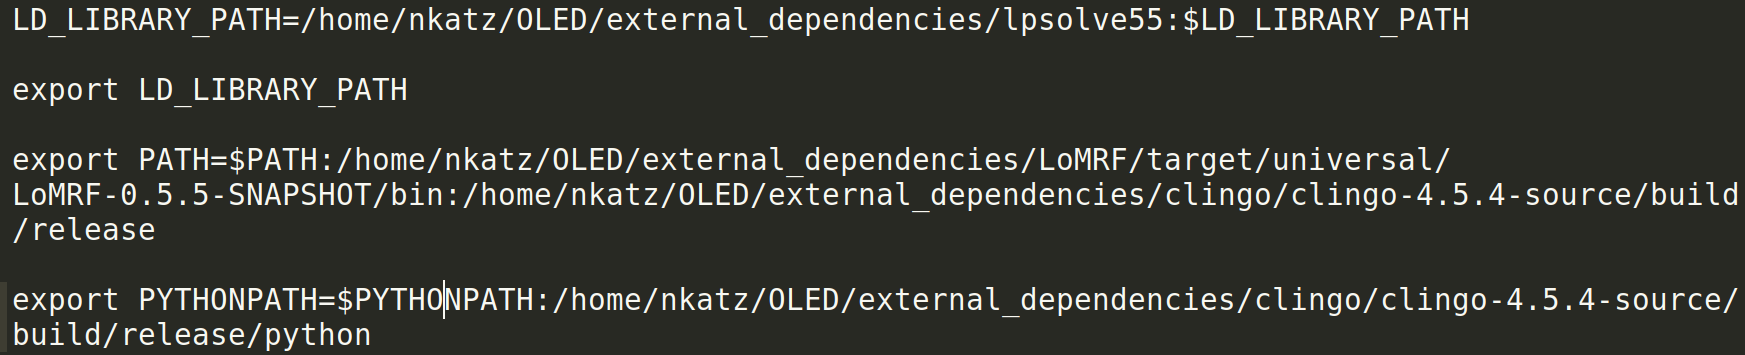
\includegraphics[width=1\textwidth]{./figures/paths}
\caption{Set paths properly at \texttt{/Home/.bashrc} or \texttt{/Home/.profile}.}%
\label{fig:install}
\end{figure}
\end{comment}

%\section{Run}
%We'll next do a test run to make sure that everything is ok. We'll use the CAVIAR\footnote{http://homepages.inf.ed.ac.uk/rbf/CAVIARDATA1/} dataset for human activity recognition. The CAVIAR dataset consists of a number of videos of actors performing a set of activities. Manual annotation (performed by the CAVIAR team) provides ground truth for two activity types. The first type corresponds to simple events and consists of the activities of a person at a certain video frame/time point, such as \emph{walking}, or \emph{standing still}. The second activity type corresponds to complex events and consists of activities that involve more than one person, e.g. two people \emph{meeting each other}, or \emph{moving together}. The goal is to recognize complex events as combinations of simple events and additional contextual knowledge, such as a person's direction and position. 

%\subsection{Download and Prepare the Data.}

%First, install MongoDB to your computer. We'll use mongo to store the data and consume it in a simulation of a streaming setting. Mongo is very easy to install, just google for specific instructions for your particular Linux distribution.  

\begin{comment}
\begin{figure}[h]
\centering
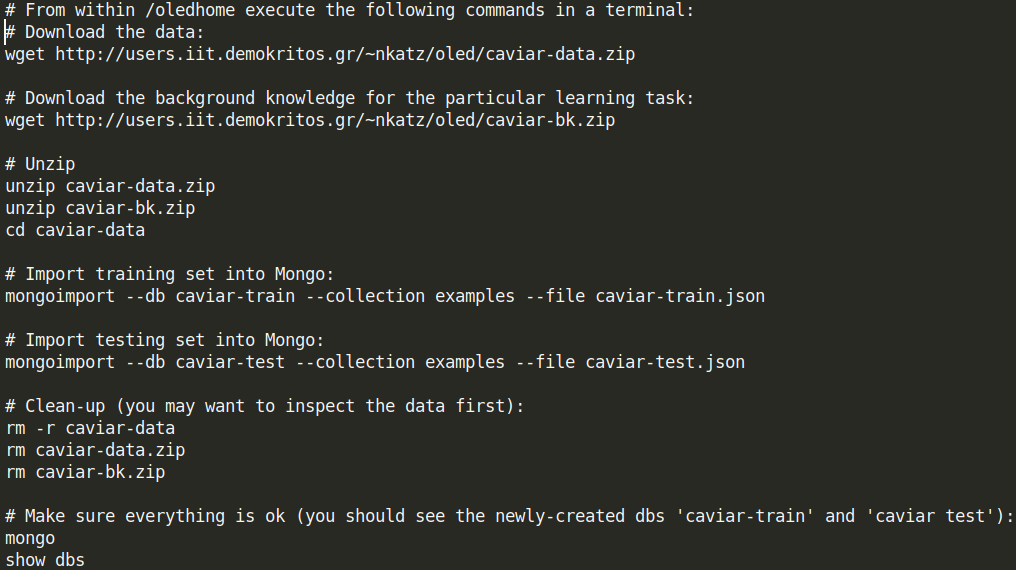
\includegraphics[width=1\textwidth]{./figures/download-caviar}
\caption{Download CAVIAR data and import it into Mongo.}%
\label{fig:caviar}
\end{figure}
\end{comment}

%Next, download the the data and import it into Mongo. Open a terminal and execute the commands shown in Figure \ref{fig:caviar}. You'll download two datasets, a fragment of CAVIAR that will be used for training (\texttt{caviar-train}) and another that will be used for testing (\texttt{caviar-test}). Subsequently, you'll import each dataset into mongo, clean-up (remove the downloaded data) and make sure that the new dbs were created as required. 

%Before cleaning up, you may wish to open the downloaded json files and inspect the data. You'll see that each entry contains three fileds: \texttt{'annotation'}, \texttt{'narrative'} and \texttt{'time'}. The \texttt{'annotation'} filed contains instances of the target complex events we wish to learn definitions for. In this example, we're learning a definition for two persons \emph{meeting each other}, therfore, \texttt{'annotation'} consists of instances of the \emph{meeting} complex event.\linebreak The \texttt{'narrative'} field consists of instances of simple events (\emph{walking}, \emph{active}, \emph{inactive} and so on) and spatiotemporal knowledge, such as persons' coordinates and direction. Each entry is a ``batch'' of data, i.e. it consists of annotation and narrative found within a temporal interval/window. The entry's \texttt{'time'} field is the first time point observed in the batch and it serves as a key to refer to that particular batch/entry.     

%Next, take a look at the background knowledge that you downloaded \linebreak (in \texttt{/caviar-bk}). It consists of three files, \texttt{ec}, \texttt{bk} and \texttt{modes}. \texttt{ec} contains the axioms of the Event Calculus. This file is optional in the general case, it is only necessary if you want to learn using the Event Calculus in the backgound knowledge (but it is necessary for the particular test OLED run that we are about to execute). \texttt{bk} is the file where the user defines some domain-specific knowledge. For the purposes of this example, \texttt{bk} contains code for calculating Euclidean distances between persons from their coordinates. Such distances are produced at learning time. All content of the \texttt{ec} and the \texttt{bk} is Answer Set Programming (ASP) code that \texttt{Clingo}, OLED's main reasoning component, is able to execute. Please consult the guide provided by the \texttt{Clingo} team\footnote{Available from \url{https://potassco.org/}, at the documentation site}. The user may use any ASP code in the \texttt{bk} file to define tasks that will be executed by \texttt{Clingo} at learning time, e.g. generating extra, non-input knowledge for the input data, or performing numerical computations via embedded Lua or Python scripts. 

%The \texttt{modes} file contains some language bias, i.e. restrictions to the syntax of predicates that may be used to form rules. OLED uses \emph{mode declarations} as a language bias (see the paper that comes with the source code, or any ILP-introductory textbook for details). in addition to the lanhuage bias, the \texttt{modes} file contains a declaration of annotation predicate signatures (via the \texttt{examplePattern/1} predicate) and input predicate signatures (via \texttt{inputPredicate/1}). The latter is the signature specification of all predicates used to pass data to the input and it is used to extract entity types during the learning process. The modes file is necessary for all learning tasks.

We are now ready to perform learning with OLED. cd to your  \ folder and run the following in a terminal:

\noindent \texttt{java -cp oled-0.1.jar app.runners.OLEDDefaultRunner \textbackslash}\\
\texttt{--inpath=<PATH TO caviar-bk FOLDER> --delta=0.00001 \textbackslash}   \\
\texttt{--prune=0.8 --target=meeting --train=caviar-train \textbackslash}\\
\texttt{--saveto=<PATH TO SOME LOCATION>/theory.lp}

To see all available command line arguments do \texttt{java -cp oled-0.1.jar -help}. The learnt hypothesis will be saved in \texttt{/oledhome/theory.lp}. You may evaluate this theory on the test set as follows: 

\noindent \texttt{java -cp oled-0.1.jar app.runners.OLEDDefaultRunner \textbackslash}\\
\texttt{--inpath=<PATH TO caviar-bk FOLDER> --target=meeting \textbackslash}   \\
\texttt{--test=caviar-test --evalth=<PATH TO theory.lp>}


\newpage
%\phantomsection
%\addcontentsline{toc}{section}{References}
\bibliographystyle{plain}
\bibliography{refs}

\end{document}
